\chapter{Popis sítě Transformer}
Transformer byl poprvé představen výzkumným týmem z Google Brain~\cite{link31} v roce 2017 v článku s názvem `Attention Is All You Need' (Pozornost je vše, co potřebujete)~\cite{link27}.
Tento článek představil novou architekturu založenou na mechanismu self-attention, který se ukázal jako velmi efektivní při zpracování sekvencí a dosáhl vynikajících výsledků v oblasti strojového překladu.

Transformer~\cite{link28}~\cite{link25} je architektura hluboké neuronové sítě, která se zaměřuje na problémy sekvence-na-sekvenci, jako je strojový překlad, generování textu nebo analýza sentimentu.
Byl vyvinut jako alternativa k rekurentním neuronovým sítím, jako je LSTM a GRU, a přinesl s sebou zásadní inovaci v oblasti zpracování přirozeného jazyka.

Hlavním stavebním prvkem Transformer sítí je self-attention mechanismus, který umožňuje modelu přidělovat váhu různým slovům v sekvenci na základě jejich vzájemného vztahu a kontextu.
Tímto způsobem si Transformer dokáže lépe poradit s dlouhodobými závislostmi v sekvencích a zachovat informace o kontextu.

Transformer se skládá z několika vrstev sítě obsahujících self-attention mechanismus a další bloky, jako jsou dopředně šířící se sítě (feed-forward) a normalizační vrstvy.
Model je trénován pomocí mechanismu nazvaného `masked multi-head attention' a optimalizován na základě ztrátové funkce, jako je například cross-entropy.

\section{Vlastnosti}
Transformer je navržen pro zpracování sekvenčních dat, včetně vět v přirozeném jazyce.
Jedním z hlavních rozdílů mezi Transformer sítěmi a RNN je právě schopnost Transformer sítí zpracovávat veškerá vstupní data najednou, zatímco RNN musí pracovat sekvenci po sekvenci.
Díky mechanismu self-attention dokáže Transformer přiřadit kontext a důležitost jednotlivým slovům v sekvenci, což umožňuje zpracování celých vět najednou.

Díky této vlastnosti má Transformer výhodu v paralelizaci, protože může zpracovávat vstupní data paralelně na větší části modelu.
To vede k výraznému zrychlení trénování modelu bez ztráty výkonu.
Oproti tomu u RNN je paralelizace složitější kvůli nutnosti zpracovávat data postupně.

Transformer také využívá techniky pozičního kódování (position encoding) pro zachycení kontextu a pozice jednotlivých slov ve vstupní sekvenci.
Pomocí mechanismu attention dokáže mapovat vztahy mezi slovy a lépe porozumět významu a vztahům ve větě.

Před-trénované modely, jako například BERT nebo GPT, jsou vytrénované na velkých datových souborech a poté mohou být doučeny (fine-tuned) na specifické úlohy.
Tyto modely představují významný pokrok v oblasti zpracování přirozeného jazyka, protože mají již naučené znalosti o kontextu a vztazích mezi slovy, což usnadňuje jejich aplikaci na různé úlohy a vede ke zlepšení výkonu.

\section{Architektura}
Architektura Transformer sítí~\ref{fig:Transformer} je založena na mechanismu self-attention, který umožňuje efektivně přiřadit kontext jednotlivým slovům (tokenům) v sekvenci.
Transformer se skládá z několika klíčových komponent, které jsou kodér (Encoder), dekodér (Decoder), Multi-head Attention a poziční kódování (Positional Encoding).

Transformer je schopen zpracovávat vstupní sekvence najednou, což umožňuje výrazně paralelizovat výpočty a urychlit trénování modelu.
Díky kombinaci self-attention, multi-head attention a dopředného šíření použité v neuronové síti je Transformer schopný efektivně zachytit vztahy mezi slovy a generovat kvalitní výstupy pro různé úlohy, včetně strojového překladu, generování textu a dalších úloh zpracování přirozeného jazyka.

\begin{figure}[H]
	\centering
	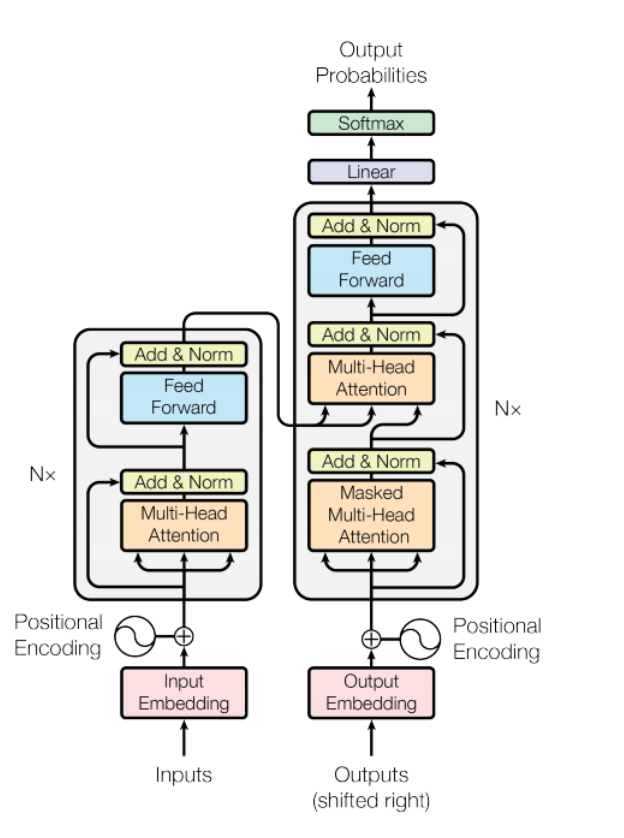
\includegraphics[width=0.6\textwidth]{Figures/transformer_enco_deco.png}
	\caption{Architektura Transformer sítí~\cite{link25}}\label{fig:Transformer}
\end{figure}

\subsection{Kodér}
Kodér (Encoder) převádí vstupní sekvenci (např.\ větu) do vektorové reprezentace.
Skládá se z několika identických vrstev, zvaných kódovacích vrstev (encoder layers).
Každá vrstva obsahuje dvě subkomponenty: multi-head self-attention mechanismus a dopředně šířící se sítě.
Self-attention mechanismus umožňuje modelu získat důležité informace o kontextu jednotlivých slov v rámci sekvence.
Neuronová síť s použitím dopředného šíření slouží k transformaci a kombinaci informací z self-attention mechanismu.

\subsection{Dekodér}
Dekodér (Decoder) generuje výstupní sekvenci (např.\ přeloženou větu) na základě zakódované vstupní sekvence.
Stejně jako kodér, dekodér se skládá z několika identických vrstev, zvaných dekódovací vrstvy (decoder layers).
Každá vrstva obsahuje tři subkomponenty: masked multi-head self-attention mechanismus, který umožňuje dekodéru vidět pouze předchozí pozice, multi-head attention mechanismus, který se zaměřuje na kódovaný kontext, a neuronovou síť pro transformaci a kombinaci informací.

\subsection{Multi-head Attention}
Attention mechanismus je klíčovou součástí sítí Transformer.
Umožňuje modelu přiřadit různou důležitost různým částem vstupní sekvence při generování výstupu.
Transformer používá multi-head attention~\ref{fig:Multi Head Attention}, což znamená, že attention mechanismus je aplikován několikrát s různými projekcemi vstupních vektorů.
To umožňuje modelu získat různé perspektivy na vztahy mezi slovy.

\begin{figure}[H]
	\centering
	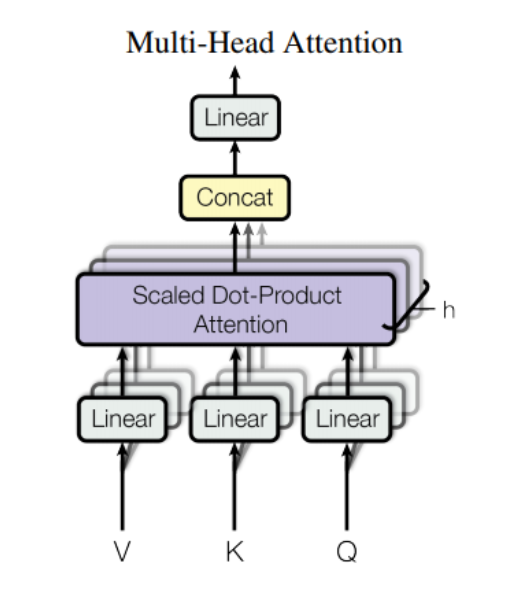
\includegraphics[width=0.6\textwidth]{Figures/multi_head_attention.png}
	\caption{Multi-head Attention~\cite{link25}}\label{fig:Multi Head Attention}
\end{figure}

Každá attention head jednotka využívá tři maticové transformace (Wq, Wk, Wv) pro dotazování (query), klíče (keys) a hodnoty (values) vstupních slov (tokenů).

Výpočet attention se provádí paralelně pro všechny attention head jednotky, což umožňuje efektivní zpracování.
Výsledky z jednotlivých attention head jednotek jsou následně spojeny a předány dále pomocí neuronové sítě využívající dopředné šíření do dalších vrstev transformace.

Tímto způsobem model může získat různé informace o vztazích a relevanci mezi slovy v rámci vstupní sekvence.
Každá attention head jednotka se může zaměřit na specifické aspekty, jako je sledování kontextuálních závislostí, vazeb mezi slovy nebo jiné relevantní informace.

\subsubsection{Počítání techniky Attention}
Transformer využívá scaled dot-product attention~\ref{fig:Scaled Dot-Product Attention} jako mechanismus pro výpočet vah mezi slovy (tokeny) vstupní sekvence.

Při výpočtu scaled dot-product attention jsou vstupní sekvence transformovány pomocí maticových transformací (Wq, Wk, Wv) na dotazovací (query), klíčové (keys) a hodnotové (values) vektory.
Poté se vypočítá podobnost (dot product) mezi dotazovým vektorem a klíčovými vektory.

\begin{figure}[H]
	\centering
	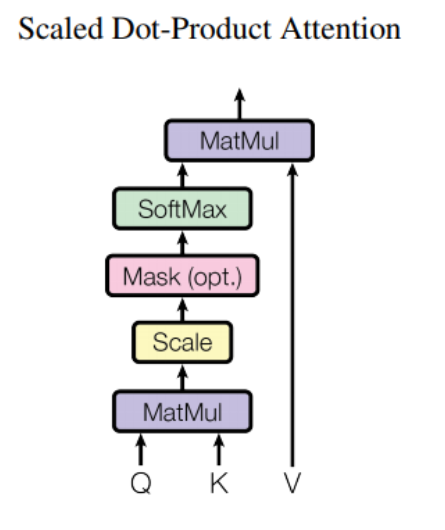
\includegraphics[width=0.6\textwidth]{Figures/scaled_product.png}
	\caption{Scaled Dot-Product Attention~\cite{link25}}\label{fig:Scaled Dot-Product Attention}
\end{figure}

Jedním z klíčových kroků je normalizace podobnosti pomocí škálování, aby se zabránilo problémům s velkými hodnotami např.\ stabilita gradientu.
Následně s využitím Softmax funkce (viz.~následující vzorec) se získávají normalizované váhy pro každý token v rámci sekvence, což reprezentuje jeho relevanci vůči ostatním tokenům.

\[Attention(Q, K, V) = softmax(QK^{T}/\sqrt[2]{d_{k}}) V\]

Následně se váženě kombinují hodnotové vektory (values) s váhami, což vytváří vektor vkládání slov pro každý token v kontextu.
Tento vektor reprezentující vkládána slova~\ref{fig:Vypocet Attention pro sekvenci} obsahuje informaci o samotném tokenu a jeho vztahu k ostatním relevantním tokenům v sekvenci.

\begin{figure}[H]
	\centering
	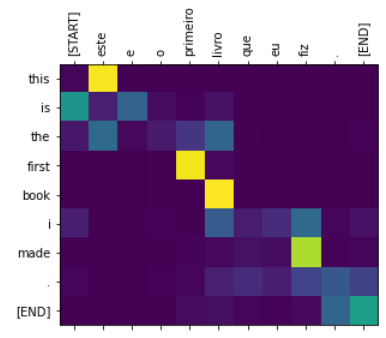
\includegraphics[width=0.6\textwidth]{Figures/attention_example.png}
	\caption{Prezentována technika Attention~\cite{link25}}\label{fig:Vypocet Attention pro sekvenci}
\end{figure}

\subsection{Poziční kódování}
Pro zachycení pořadí slov v sekvenci používá Transformer poziční kódování (positional encoding)~\cite{link38}.
Jedná se o speciální vektorovou reprezentaci, která je přidána ke vstupním slovům (tokenům) a poskytuje informaci o jejich pozici v sekvenci.
Tímto způsobem se zachovává informace o pořadí slov i při zpracování vstupu bez rekurentního propojení.

\subsubsection{Vstupní data}
Ve vstupním procesu Transformer sítí jsou slova reprezentována pomocí techniky vkládání slov, která je často založena na před trénovaných slovních vektorech.
Tyto vektory mají pevnou dimenzi, která se obvykle pohybuje v rozmezí desítek až stovek.

Technika vkládání slov zachycuje významové vztahy mezi slovy, ale nezahrnuje informaci o jejich pozici v sekvenci.
Proto je k zachování informace o pořadí slov v Transformer sítí použita technika nazývaná poziční kódování~\ref{fig:Zobrazeni positional encodingu pro 128D vektor} (viz.~následující~vzorce).

Pozici slov (tokenů) v sekvenci určuje kombinace hodnot vektoru pozičního kódování a vektoru reprezentující vkládána slova.
Tyto informace jsou následně vstupem do kodéru a dekodéru Transformer sítí, který na základě nich provádí operace techniky attention a generuje výstupní sekvenci.

\[PE_{(pos,2i)} = \sin(pos/10000^{2i/d_{model}})\]
\[PE_{(pos,2i+1)} = \cos(pos/10000^{2i/d_{model}})\]

\begin{figure}[H]
	\centering
	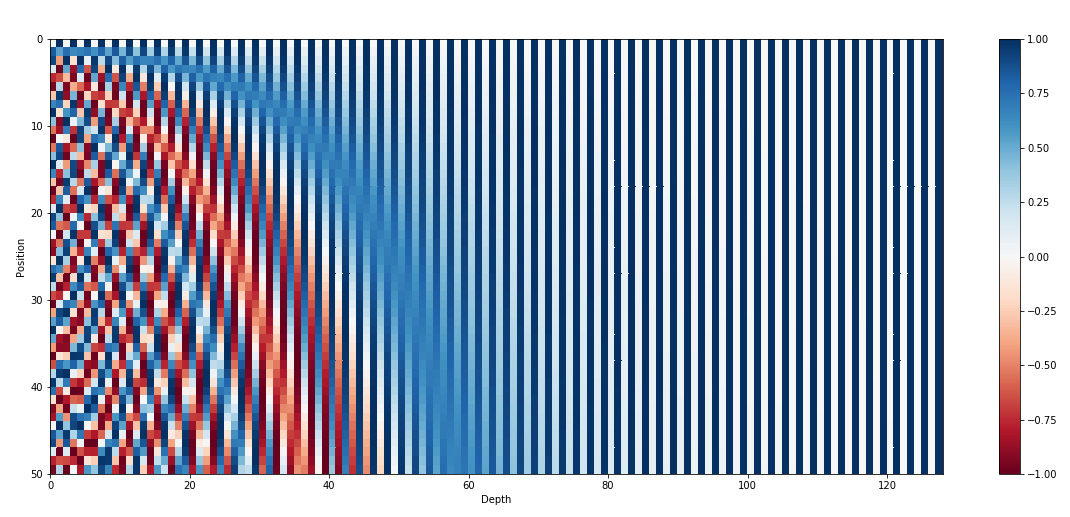
\includegraphics[width=0.6\textwidth]{Figures/positional_encoding.png}
	\caption{Zobrazení Positional Encoding techniky pro 128D vektor~\cite{link38}}\label{fig:Zobrazeni positional encodingu pro 128D vektor}
\end{figure}

\section{Trénování modelu}
Transformer sítě se často učí pod samo dohledem (self-supervised), který kombinuje volné učení (unsupervised) na velkém datovém souboru a následně doučeny (fine-tuned) pomocí učení pod dohledem (supervised).

Při volném učení je Transformer modelu prezentováno velké množství neoznačených dat, například textové korpusy získané z Internetu, které jsou bohaté na přirozený jazyk.
Model se učí predikovat následující slovo v sekvenci, rekonstruovat chybějící části vstupní sekvence nebo provádět jiné úlohy, které vyžadují porozumění kontextu a vztahům mezi slovy.
Tímto učením se model naučí efektivně zpracovávat textová data, zachytávat jazykové vzorce a získávat všeobecné znalosti o vztazích mezi slovy.

Po volném učení trénování je model doučen pomocí dohledového učení na menším označeném datasetu specifickým pro konkrétní úlohu.
Například pro sentimentální analýzu se používá dataset obsahující texty s označeným sentimentem, pro modelování jazyka se používá textový dataset s označenými sekvencemi.

Tímto kombinovaným přístupem se dosahuje dobrého výkonu na konkrétních úlohách zpracování přirozeného jazyka, jako je sentimentální analýza, generování následujících vět, modelování jazyka nebo odpovídání na otázky.
Transformer sítě díky své schopnosti zachycovat kontext a vztahy mezi slovy dosahují v těchto úlohách často nejlepšího (state-of-the-art) výkonu.

\section{Aplikování}
Transformer sítě se ukázaly jako velmi úspěšné v oblasti zpracování přirozeného jazyka a na mnoha úlohách, včetně strojového překladu a časové závislých (time series) předpovědí.
Jejich schopnost zachycovat kontext a vztahy mezi slovy a efektivně zpracovávat sekvence je velmi výhodná pro tyto úlohy.

Nicméně, Transformer sítě mají široké možnosti využití i v jiných oblastech.
Před-trénované modely, jako je GPT-2, se ukázaly jako úspěšné v generování textu, ať už jde o tvorbu nových článků, dialogů, nebo dokonce celých dokumentů.
Díky schopnosti zachycovat kontext a syntaktické struktury vět dokáží tyto modely produkovat texty s vysokou kvalitou a přirozeností.

Transformer sítě se také osvědčily v oblasti analýzy biologických sekvencí, kde jsou schopny zpracovávat sekvence DNA nebo proteinů a hledat vzorce a vztahy mezi nimi.
V oblasti porozumění videím se Transformer sítě využívají k analýze videí a extrakci informací z video sekvencí.

Dalším zajímavým příkladem je využití Transformer sítí v šachových algoritmech, kde mohou být před-trénované modely, jako je GPT-2, doučeny na hrání šachu.
Tyto modely se naučí strategie a pravidla hry a mohou dosahovat vysoké úrovně ve hře proti lidským hráčům.

Transformer sítě tedy nabízejí široké spektrum využití a mohou být adaptovány na různé oblasti, kde je důležité zpracovávat sekvence dat a zachycovat jejich vztahy a strukturu.

\section{BERT}
BERT~(Bidirectional~Encoder~Representations~from~Transformers)~\cite{link29}~\ref{fig:BERT model} je architektura založená na Transformer modelu pro zpracování přirozeného jazyka (NLP).
Byl vytvořen týmem Google~Brain~\cite{link31} a poprvé publikován v roce 2018.

BERT přinesl významný pokrok v oblasti NLP a dosáhl několika nejlepších (state-of-the-art) výsledků v různých NLP úlohách.
Jeho klíčovou vlastností je schopnost zachytit vztahy mezi slovy a jejich kontextem v obou směrech, tedy v předcházejícím i následujícím kontextu.
Tímto způsobem BERT vytváří velmi bohaté a reprezentativní vektorové reprezentace slov a vět.

Díky své schopnosti zachytit jazykový kontext se BERT stal populárním a v roce 2020 byl hojně využíván ve strojovém překladu z anglického jazyka do jiných jazyků.
Jeho před-trénované váhy a modelové znalosti umožňují efektivní adaptaci na různé úlohy pomocí doučující techniky.

BERT otevřel cestu pro další vylepšené architektury v oblasti NLP.\@
Tato architektura se stala důležitým nástrojem pro různé úlohy zpracování přirozeného jazyka, včetně strojového překladu, rozpoznávání entit, sentiment analýzy a dalších.

Původně veřejně publikován BERT má dva typy konfigurace pro sdílení.

\begin{itemize}
\item BERT BASE, který obsahuje 12 enkodéru s 12ti self-attention head jednotkami
\item BERT LARGE s 24 enkodéry a 16ti self-attention head jednotkami
\end{itemize}

BERT je před-trénován na neoznačených (unsupervised) jazykových reprezentacích, což znamená, že trénovací data, na kterých je trénován, nejsou specificky označena pro určitý výstup.
Místo toho jsou použity rozsáhlé textové korpusy, které byly získány ze stránek jako jsou např. Wikipedie a BooksCorpus, které obsahují obecný textový materiál z různých zdrojů.

Díky před trénování na rozsáhlých a různorodých textových korpusů BERT získává obecné jazykové znalosti, které mu umožňují lépe porozumět a reprezentovat různé textové vstupy.
Tato schopnost představuje výhodu při aplikacích NLP, kde je modelu potřeba porozumět a zachytit různé jazykové nuance a vztahy.

BERT bere v potaz kontext slova, což mu umožňuje rozlišovat význam slova v závislosti na jeho kontextu.
Rozdíl ve významu slova `koruna' v následujících větách by měl být reflektován v reprezentaci chování BERT modelu.

\begin{itemize}
\item Česká koruna se propadla nejvíce v historii ČR.
\item V korunách stromů sedí ptáci.
\item Král nosí korunu.
\end{itemize}

BERT je obousměrným (bidirectional) modelem, což znamená, že bere v potaz kontext slova z obou směrů.
Tato vlastnost je dosažena pomocí mechanismu nazývaného maskované modelování jazyka (masked language modeling), kdy BERT se učí předpovídat chybějící slova v textu na základě kontextu, který zahrnuje jak slova před nimi, tak slova za nimi.

Díky obousměrnému zohledňování kontextu je BERT schopen zachytit slovní vztahy a významy ve větách, které jsou důležité pro porozumění celému textu.
Tím se odstraňuje omezení jednosměrných (unidirectional) modelů, které sledují kontext pouze z jednoho směru.
Obousměrný přístup BERTa umožňuje lépe modelovat závislosti mezi slovy a vytvářet kontextuální reprezentace jednotlivých slov na základě celé věty.

\begin{figure}[H]
	\centering
	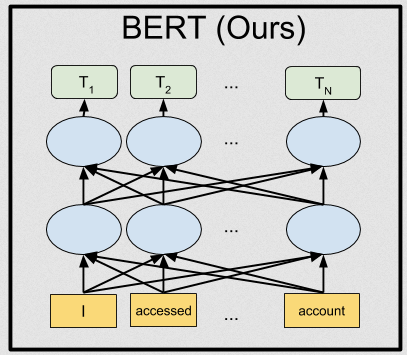
\includegraphics[width=0.6\textwidth]{Figures/BERT.png}
	\caption{BERT model~\cite{link24}}\label{fig:BERT model}
\end{figure}

\subsection{Ukázka obousměrného přístupu}
V následující větě `Já jsem Honza' BERT s obousměrným přístupem je schopen zachytit vztah slova `jsem' nejen k předchozímu slovu `Já', ale také k následujícímu slovu `Honza'.
Díky své schopnosti zohledňovat kontext z obou směrů dokáže BERT lépe porozumět vztahům mezi slovy ve větě.

V případě jednosměrného modelu by pouze kontext předcházející slovu `jsem' nebo kontext následující slova `jsem' byl brán v úvahu při modelování vztahu s tímto slovem.
To by mohlo vést k omezenému porozumění celému kontextu věty.

Díky schopnosti BERTa zohledňovat kontext ze všech stran je schopen zachytit významy obou slov `Já' a `Honza' a lépe reprezentovat jejich vzájemný vztah ve větě `Já jsem Honza'.
Tímto způsobem BERT dokáže lépe porozumět významům jednotlivých slov a jejich vztahům v celém kontextu věty.

Jednosměrný přístup, který je běžně používán v tradičních jazykových modelech, neumožňuje předvídat budoucí slova na základě slov, která jej předcházela a následovala.
Tím pádem by při jednosměrném modelování nebylo možné získat úplný kontext věty.

BERT řeší tento problém pomocí techniky maskování (masking)~\ref{fig:BERT maskovani}.
Při trénování BERTa jsou náhodně vybraná slova vstupního textu maskována a následně je model trénován na předpovídání těchto zakrytých slov na základě okolního kontextu.
Tímto způsobem BERT získává schopnost porozumět kontextu celé věty a naučit se předpovídat nejen slova na základě předchozích, ale i na základě budoucích slov, která jsou v daném kontextu maskována.

\begin{figure}[H]
	\centering
	
\includegraphics[width=1\textwidth]{Figures/BERT_bi.png}
	\caption{BERT případ maskování~\cite{link24}}\label{fig:BERT maskovani}
\end{figure}

Technika maskování slov ve vstupním textu a následná predikce těchto slov je známá už delší dobu.
Co je unikátní u BERTa, je jeho schopnost efektivně využívat tuto techniku v kombinaci s obousměrným kontextovým modelováním.

Co se týče porozumění vztahům mezi větami, BERT má v sobě zakódovanou informaci o vzájemném vztahu dvou vět v tzv.\ segmentovém vektoru (segment embedding vector).
Segmentový vektor~\ref{fig:BERT priklad sekvence} je část reprezentace vstupního textu, která specifikuje, které slova a věty patří do kterých segmentů.
BERT je tak schopen rozpoznat, zda věta `A' následuje po větě `B' nebo naopak.

\begin{figure}[H]
	\centering
	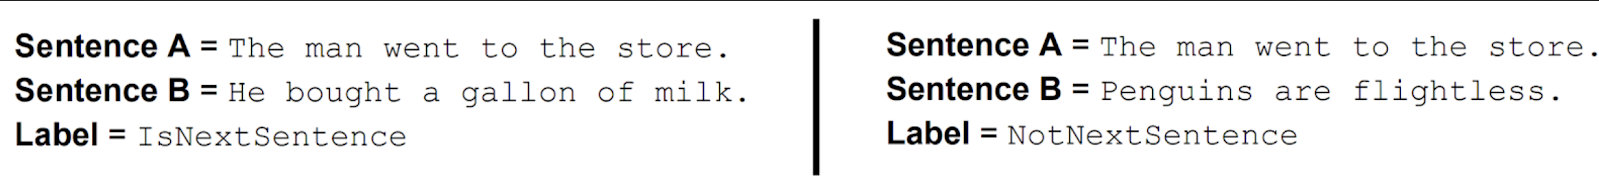
\includegraphics[width=1\textwidth]{Figures/BERT_sequence.png}
	\caption{BERT příklad sekvence~\cite{link24}}\label{fig:BERT priklad sekvence}
\end{figure}

\subsection{Využití}
Jedna z výhod Transformer sítí je možnost využití před-trénovaných modelů pro různé úlohy zpracování přirozeného jazyka.

Před-trénované modely jako je BERT jsou natrénovány na obrovských množstvích textových dat a jsou schopny zachytit bohaté vztahy mezi slovy a kontextem.
Tyto modely jsou takovým druhem jazykového modelu, který vytváří vektorové reprezentace slov a vět na základě jejich kontextu.

Pomocí techniky doučení je možné před-trénovaný model BERT přizpůsobit na specifický úkol, například pro rozpoznávání sentimentu, strojový překlad nebo jiné úlohy zpracování přirozeného jazyka.
Při doučování se upravují pouze některé části modelu, zatímco váhy a znalosti z před trénované fáze zůstávají zachovány.

\endinput